\subsubsection{Terrapene --- Box Turtles}
\begin{center}
\begin{longtabu} to \textwidth {| | p{3.5cm} | X | |}

	\hline
	Taxonomy/Ancestry &
	a member of the subfamily emydinae. 12 taxa over 4 species. Terrapene originally coined as genus separate from Emys for species w/ sternun separated into 2-3 divisions which can move independently.
	
	they appear abruptly in the fossil record in modern form, implying they are a generalist species able to survive under a wide variety of conditions. older fossils have been found in Nebraska dating back to the Miocene (15 Mya). only recognized extinct subspecies dates from Pliocene and was much larger than other species.
	
	\begin{center} 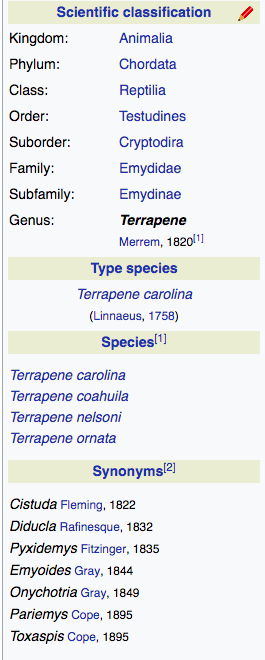
\includegraphics[scale=0.25]{testudines/emydidae/terrapene/tax} \end{center}
	 \\
	\hline
	Size & 
	10-22cm (4-9 in)
	\\
	\hline
	Color &
	females usually have yellowish-brown eyes, while males typically have red or orange eyes.
	 \\
	\hline
	Anatomy &
	\begin{itemize}[noitemsep]
		\item distinguished by domed shell which is hinged at the bottom
			\begin{itemize}[noitemsep]
				\item allows animal to close shell tightly to escape predators
			\end{itemize}
		\item item avg. lifespan of 50 yrs, but many can live past 100. once maturity is reached, the chances of death do not seem to increase w/ age.
		\item age can be roughly estimated by counting growth rings on scutes, but estimates may be inaccurate b/c the plastron is worn smooth over time.
	\end{itemize}
	 \\
	\hline
	Dimorphism & 
	Males have concave area on plastron centered beneath hinge.
	\\
	\hline
	Behavior & 
	\begin{itemize}[noitemsep]
		\item defend selves from predation by hiding, closing shell, and biting, but are vulnerable to surprise attacks and persistent gnawing/pecking
		\item tend to move further into woods prior to hibernation
	\end{itemize}
	\\
	\hline
	Habitat & 
	\begin{itemize}[noitemsep]
		\item no standard habitat, but generally found in mesic woodlands
		\item \emph{T. ornata} can be found in grasslands
		\item desert box turtle can also be found in semidesert w/ rainfall predominantly in summer
		\item Coahuilan box turtles found only in region characterized by marshes, permanent presence of water, and cacti
	\end{itemize}
	\\
	\hline
	Distribution & 
	native to N. America, where the species w/ the widest range, the common box turtle, is found in the US and Mexico. the ornate box turtle is endemic to south-central and southwestern US/adjacent Mexico, the spotted box turtle is endemic to northwestern Mexico, and the Coahuilan box turtle found only in Cuatro Cienegas Basin in Coahuila, Mexico.
	\\
	\hline
	Feeding Ecology & 
	an omnivore w/ a varied diet, it eats anything it can catch. invertebrates/insects = principal component but diet also consists of vegetation. the diet can be amended w/ fruits. at times, it eats poisonous mushrooms, making its meat dangerous for humans.
	\\
	\hline
	Reproductive Biology & 
	relatively slow reproducers, they reach sexual maturity only after 4-5 yrs. females can store viable sperm in the oviducts for up to 4 yrs. they mate from may-october and lay elliptical, leathery eggs in flask-shaped holes 3-4 in deep in warm, sunny soil. they may have more than 1 clutch a yr, w/ avg. clutch size being larger in northern populations and ranging from 1-7 eggs. incubation takes 2-3 months. infant mortality is high, since the shell is weaker. infants may overwinter in the nest.
	\\
	\hline
	Ecological Role &
	
	\\
	\hline
	Conservation Status & 
	\begin{itemize}[noitemsep]
	\item 1 EN; 1 V; 1 NT; 1 DD
	\item Often taken as or bred as pets
		\begin{itemize}[noitemsep]
			\item Easily stressed and require more care than is generally thought
			\item Require outdoor enclosure and constant exposure to sun
			\item Recommended to buy captive bred to reduce pressure on wild populations
		\end{itemize}
	\item Some states prohibit collecting wild turtles or require permits to keep them
	\item State reptile of N. Carolina, Tennessee, Missouri, and Kansas
	\end{itemize}
	\\
	\hline
\end{longtabu}
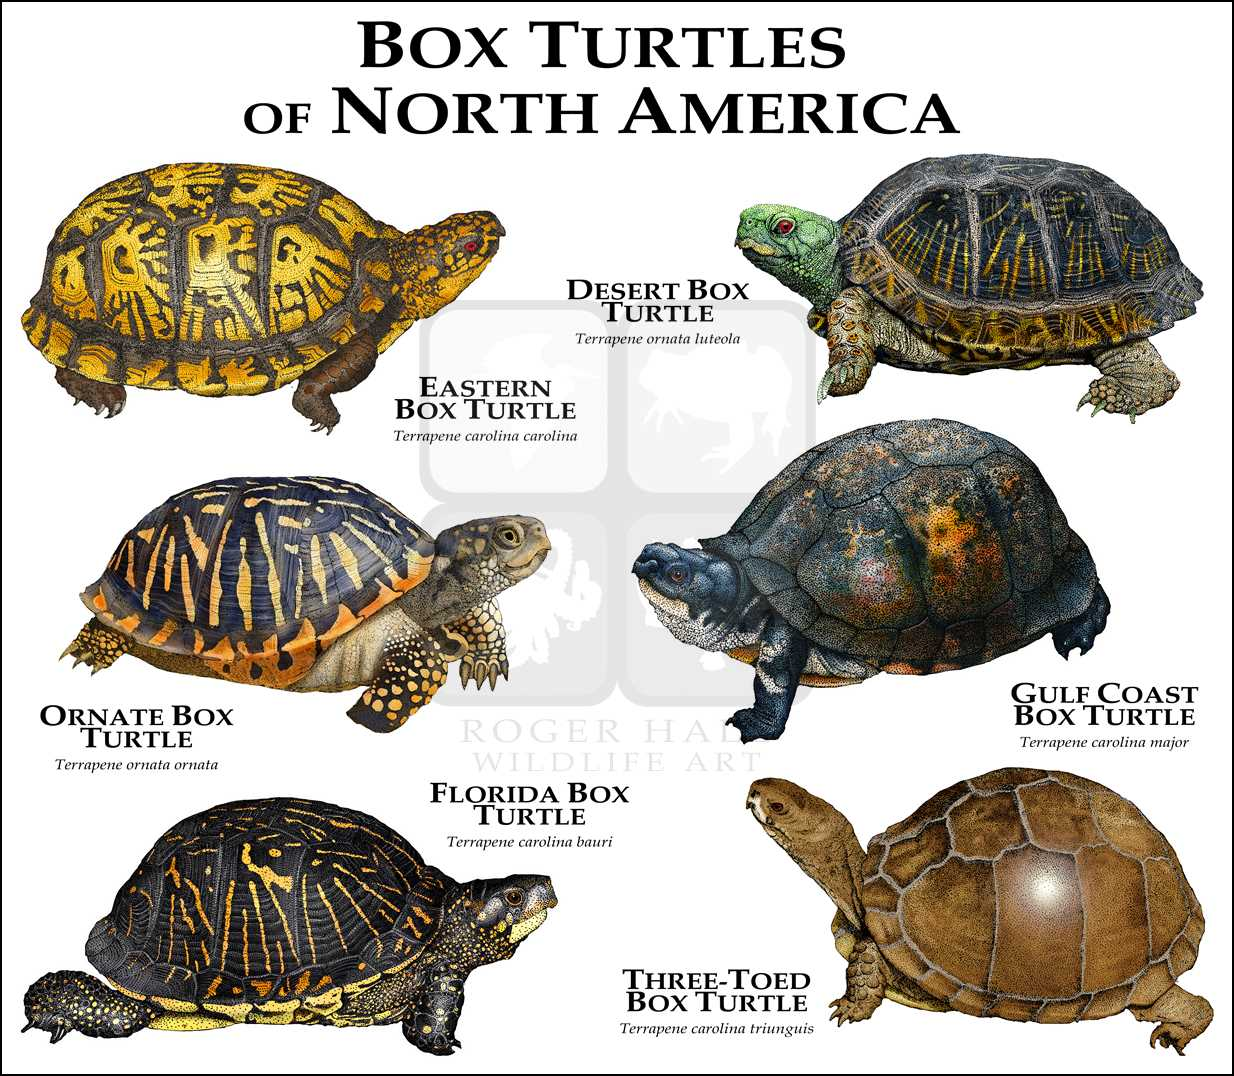
\includegraphics{testudines/emydidae/terrapene/box}
\end{center}